%===========================================================================
%	III. Actual State Analysis
%===========================================================================

As stated in the \nameref{chap:introduction} chapter, the project is conducted based on a preexisting data pipeline solution where DataOps is to be enabled, including a holistic DataOps testing framework. This chapter performs an actual state analysis, describing the superordinate data analytics use case as well as the data pipeline specification prior to the project. The resulting aspects will then be used for the testing framework specification and reimplementation process.

\section{General Information}
The data pipeline at hand is four-stage pipeline that creates a \acf{mba} for \ac{bi} and reporting purposes. \ac{mba} is one of the key techniques used by large retailers to uncover associations between items. It works by looking for combinations of items that occur together frequently in transactions \cite[1]{Chen2005}. The specific \ac{mba} performed at the end of this data pipeline provides two kinds of information. First, it describes item sets that are frequently purchased together. Specifically, the higher the \textit{support} of an item set, the higher the probability that these items are purchased together. The \textit{Apriori} algorithm is a widely used method to accomplish this \cite[12\psq]{Wu2008}. Second, the \ac{mba} calculates other association metrics (i.e., \textit{confidence} and \textit{lift}) of the item sets, allowing for backed decision-making with regard to marketing campaigns, inventory stock-up, etc.

\acp{mba} are based on a large amount of \ac{pos} data. These data need to be integrated by means of the analytics engine requirements in order to be used for \ac{mba} purposes.

\section{Analytics Solution Components}
The data pipeline consists of various infrastructural and technical components. This also includes the input and output formats of the analyses. These components are described in the following.

\subsection{\acs{mba} Engine: Python Library \texttt{mlxtend}}
The Python library \texttt{mlxtend} provides functions that are required for conducting the previously described \ac{mba}. \texttt{mlxtend.apriori} conducts the analysis of frequent item sets. These are used for the second step, where \texttt{mlxtend.association\_rules} is leveraged to calculate confidence and lift metrics \cite{mlxtend} for all item sets with support > 5\%. Currently, the resulting associations are filtered such that only those with a high lift (> 6) and high confidence (> 0.8) are provided. The result is a Microsoft Excel spreadsheet document which lists all analytically promising item sets.

For better distinction between the actual association of the products, the \ac{mba} engine performs two analyses. Technically, they perform identically but the first analysis only considers items that are classified as food. The second analysis performs by only looking at non-food items. Thus, the analysis does not take cross-category associations into account, as they might be random and complicated to take advantage of.

The \texttt{mlxtend} library works with so-called data frames which are typically managed by another Python library, \texttt{pandas} \cite{pandas}. The \ac{mba} algorithms require a data frame that flags what kinds of sub-categories of products (both food and non-food items) were purchased in every considered transaction. Thus, to provide these pieces of information, \texttt{pandas} requires an input of semi-structured data \cite{pandas} where the following requirements are satisfied:

\begin{itemize}
	\item each individual transactions can be identified: \texttt{InvoiceNo} attribute for each purchase
	\item each individual item is sub-categorized: \texttt{Description} attribute for each purchase
	\item each individual item is categorized (food or non-food): \texttt{ItemType} attribute for each purchase
	\item each individual purchase shows if and how much of an item was purchased: \texttt{Quantity} attribute
\end{itemize}

All these requirements can be satisfied by providing a single \ac{csv} file which contains an arbitrary number of transactions. Based on the transaction information, the \ac{mba} is conducted.


\subsection{Input Data: \textit{\acs{arts} \acs{pos}Log 6} Standard}
Transaction data is usually provided to the customer through a receipt that is printed out at the register. This data can also be leveraged for \ac{mba}. Since multiple registers across multiple branches of a retail company produce a large number of individual receipts every day, the format of those \ac{pos} data needs to be unified. Additionally, the data needs to be centralized such that cross-branch \acp{mba} are possible.

A widely used \ac{pos} standard is the \textit{\ac{pos}Log 6} standard by the \ac{arts}. It is used by many established register systems. It is saved in \ac{xml} format and contains the same information that is usually provided on a print-out receipt \cite{poslog}, i.e., general transaction information (e.g., name and address of retail branch, cashier's name, currency) as well as information on each item purchased (category, brand name, quantity, price, etc.). The provided information allows to find out the required attributes for \ac{mba}.

An exemplary \ac{xml} code snippet in \ac{pos}Log format for the current solution looks as follows:

\begin{longlisting}
	\inputminted{xml}{main-matter/src/3-poslog.xml}
	\caption{Sample \acs{pos}Log \acs{xml} File}
	\label{src:3-poslog}
\end{longlisting}

\subsection{Data Location: \textit{\acs{aws} \acs{s3} Data Bucket}} \label{sec:3-2-data-lake}
In a real-life retail scenario, the individual \ac{pos} data of each branch are consequently uploaded to the branches' data infrastructure. Each day at end of business, this data needs to be provided to the global \ac{mba} engine. This is why the data is compressed into a single ZIP archive, identified by branch name and date stamp, and uploaded to the landing zone of the global retail company data lake. This data lake is realized with an \ac{aws} \ac{s3} data bucket, a server-less data storage solution \cite{s3}. The data lake structure can be seen in Figure \ref{fig:3-data-lake}.

\newpage

\begin{figure}[h!]
	\centering
	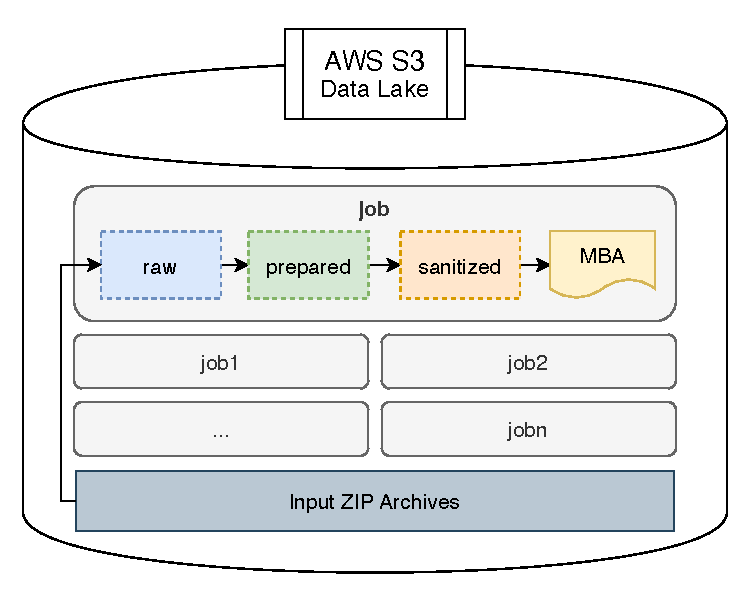
\includegraphics[width=0.67\linewidth]{main-matter/img/3-data-lake.pdf}
	\caption{Preliminary Data Lake Structure}
	\label{fig:3-data-lake}
\end{figure}

For the data analytics pipeline which integrates the data and performs the actual \ac{mba}, the landing zone of production-grade data (as described in the previous paragraph) is considered the entry point. It receives the previously mentioned \ac{pos}Log ZIP archives. It also contains the job sub area which contains all analysis jobs, e.g., an \ac{mba} every day after receiving new data. Each job area is again divided into sub areas which are used as intermediate destinations for the individual data pipeline stages, while the resulting \ac{mba} Excel spreadsheet file is uploaded to the root of its job area.

\subsection{Centralized Data Processing Engine: \textit{\acs{aws} Athena} Serverless \acs{sql} Database}

It is desirable that a global \ac{mba} engine performs the analysis rather than every branch performing their own analyses since this might lead to inconsistencies between the individual results. Therefore, the data lake is not only used for storage purposes, but is rather the actual area where the analysis is performed based on the contents in its raw zone. Considering structure, all \ac{pos} data across all branches is expected to be identical, which means that all data can be normalized and synthesized in the same way, allowing the data to be ingested into a relational database table for querying purposes.

\ac{aws} Athena makes use of the \ac{s3} data lake and does not require additional data storage resources. It rather considers a specific area of the \ac{s3} bucket its data source and can query against it using traditional \ac{sql} \cite{athena}. The query results are represented in \ac{csv} format that can be used by the \ac{mba} engine to perform its analyses.

The query for the information required by the MBA looks as follows:

\begin{listing}[H]
	\inputminted{sql}{main-matter/src/3-athena-query.sql}
	\caption{\acs{sql} Query for Required \acs{mba} Information}
	\label{src:3-athena-query}
\end{listing}

This yields an output of the following format:
\begin{table}[h!]
	\centering
	\begin{tabular}{r|ll}
		\textbf{Attribute}      & \textbf{Data Type}  & \textbf{Corresponding \acs{json} Attribute}  \\ \hline \\[-1em]
		\textbf{\texttt{SequenceNumber}} & \texttt{bigint}     & \texttt{SequenceNumber}               \\ \\[-1em]
		\textbf{\texttt{Description}}    & \texttt{string}     & \texttt{ItemCategory}                 \\ \\[-1em]
		\textbf{\texttt{ItemType}}       & \texttt{char} (\texttt{F}/\texttt{N}) & \texttt{ItemID} (first character)     \\ \\[-1em]
		\textbf{\texttt{Quantity}}       & \texttt{int}        & \texttt{Quantity}                    
	\end{tabular}
	\caption{\acs{csv} Output Format}
	\label{tab:3-csv-format}
\end{table}

Using an entire external service (i.e., \ac{aws} Athena) might appear to have a high overhead but could be leveraged especially in situations where the \ac{mba} input requires different data. In that case, only an \ac{sql} query would need to be updated, as opposed to the entire source code of one or multiple stages of the pipeline. In case the MBA does not change its requirements, it might be possible to handle the \ac{xml}-to-\ac{csv} conversion and reduction internally. The current solution applies \ac{aws} Athena for simplicity reasons.

\section{Data Pipeline}
The goal of the data pipeline is to integrate the input data (i.e., the \ac{pos}Log \ac{xml} files) and preparing the required accumulated, \ac{csv}-formatted data for the actual \ac{mba}. This process is divided into three preparatory data integration stages and followed by the fourth and final \ac{mba} stage.

In theory, a data pipeline can be understood as a \ac{dag}, since it defines a specific flow direction as well as a beginning and an end of one analytics period. The pipeline \ac{dag} at hand is technically encapsulated inside the \textit{Apache Airflow} workflow software. It makes use of \acp{dag} to define, manage, and operate (analytical) workflows. Airflow is Python-driven and provides a \ac{ui} for real-time monitoring purposes \cite{airflow}, which makes it suitable for data analytics processes. It is important to mention that, currently, Airflow does not only orchestrate the analysis, but rather performs it. All analytics scripts are directly written into Airflow. The terms \textit{pipeline} and \textit{\ac{dag}} can be used interchangeably in the current state of the analytics solution. Its general structure is presented in Figure \ref{fig:3-data-pipeline} below.

\begin{figure}[h!]
	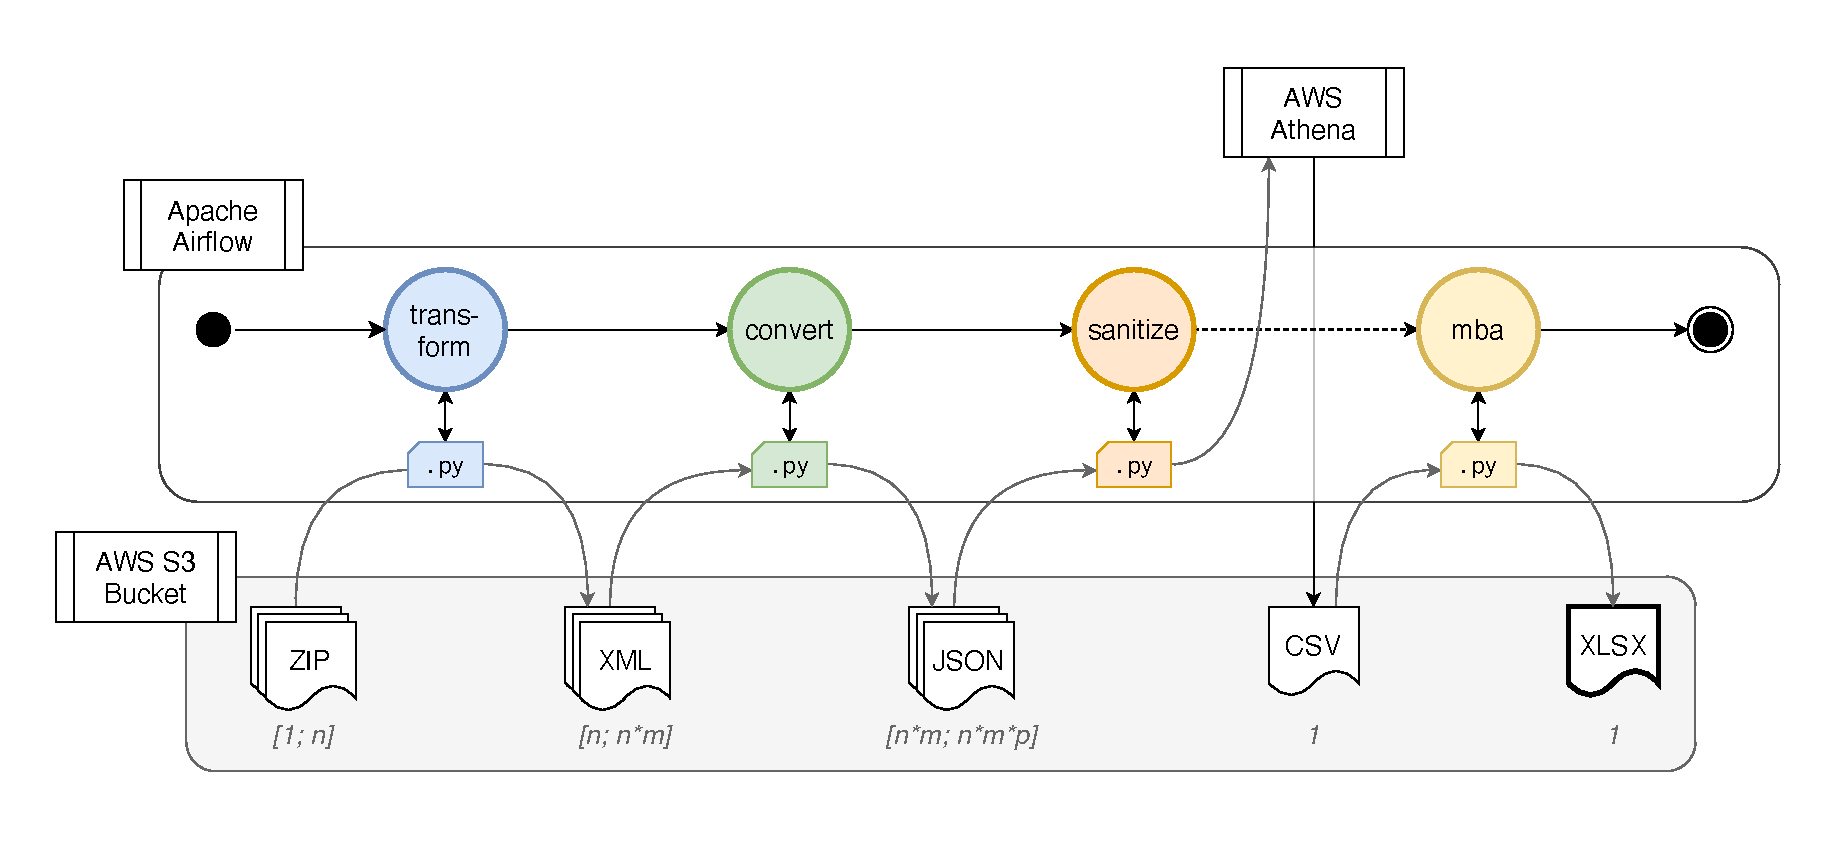
\includegraphics[width=\linewidth]{main-matter/img/3-3-data-pipeline.pdf}
	\caption{Data Pipeline Overview}
	\label{fig:3-data-pipeline}	
\end{figure}

As shown in Figure \ref{fig:3-data-pipeline}, the Transformation Stage scans the pre-defined data lake landing zone for ZIP archives. It decompresses the ZIP archives and loads all \ac{xml} files into a designated raw-file directory of the job-specific data lake space. The Conversion Stage takes the resulting data and prepares it for a serverless database integration, realized with \ac{aws} Athena. The Sanitization Stage queries the resulting table for the attributes required by the \ac{mba} engine. The query result is exported in \ac{csv} format and provided to the \ac{mba} engine, which performs the analysis in its designated \ac{mba} Stage, which represents the final stage of the data pipeline.

\newpage

\subsection{Transformation Stage}
Figure \ref{fig:3-transform} visualizes the Transformation Stage.

\begin{figure}[h!]
	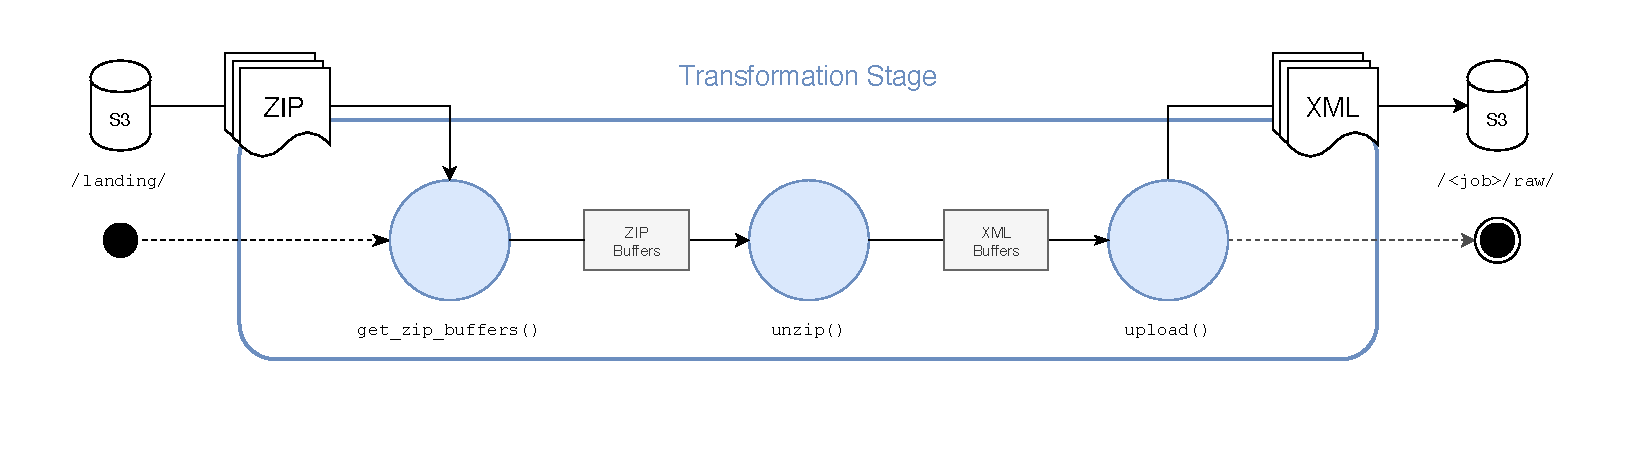
\includegraphics[width=\linewidth]{main-matter/img/3-3-1-transform}
	\caption{Transformation Stage of the Data Pipeline}
	\label{fig:3-transform}	
\end{figure}

The archived \ac{xml} data needs to be decompressed such that its contents can be read out and analyzed. In order not to contaminate the landing zone of the data lake, the data is simply decompressed and uploaded to a raw-file directory within the designated job data lake space. The \ac{xml} data is nested, which is not suited for the direct integration into a relational database table, which is why the data needs to be converted in the next stage.

\subsection{Conversion Stage} \label{sec:3-3-conversion}
Figure \ref{fig:3-convert} visualizes the Conversion Stage.

\begin{figure}[h!]
	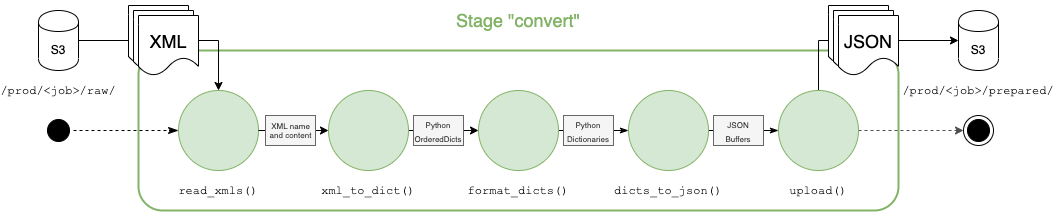
\includegraphics[width=\linewidth]{main-matter/img/3-3-2-convert}
	\caption{Conversion Stage of the Data Pipeline}
	\label{fig:3-convert}	
\end{figure}

The \ac{xml} files contain transaction-level information where the individual purchases are nested into. The \ac{mba} engine requires purchase-level information with a transaction reference which means that the \ac{xml} data needs to be redundantly converted. The resulting data should still contain transaction information, but a single data entity needs to provide information on a single purchase within the referenced transaction and shall not be nested.

Before this conversion can take place, the \ac{xml} data needs to be made processable in Python. Here, the \texttt{xmltodict} library is leveraged. The resulting Python dictionaries reflect the structure of the \ac{xml} file. To achieve the goal of purchase-level dictionaries, each purchase in a dictionary creates its own dictionary and also gets all transaction information provided. This process is visualized in Figure \ref{fig:3-convert-process}. %TODO: Reference JSON file format in Appendix

\begin{figure}[h!]
	\centering
	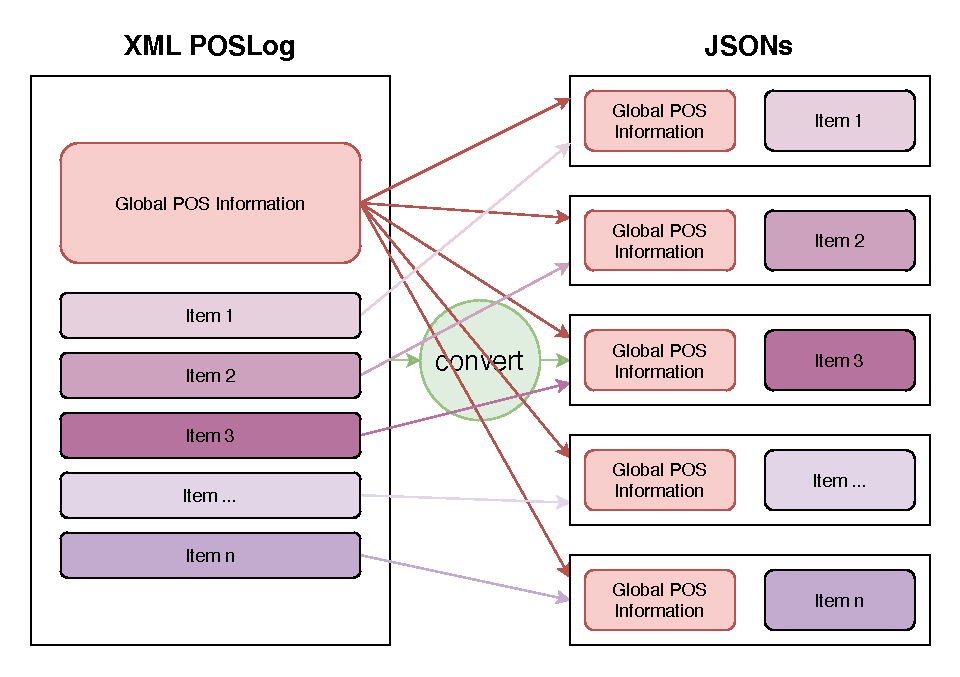
\includegraphics[width=0.67\linewidth]{main-matter/img/3-convert-process.pdf}
	\caption{Conversion of Nested \acs{pos}Log \acs{xml} Files}
	\label{fig:3-convert-process}
\end{figure}

In simple terms, each new dictionary can be seen as a receipt for a single purchase since it contains all global transaction information as well as sale information for a single item.

The final step of this stage is to provide the data in a format that can be queried against using \ac{aws} Athena \ac{sql} queries. Per its documentation, \ac{json} is a supported data format \cite{athena}. Thus, each dictionary is exported as its own \ac{json} file to a prepared-file directory within the designated job data lake space. An example output \ac{json} file can be seen below.

\begin{longlisting}
	\inputminted{json}{main-matter/src/3-json.json}
	\caption{Samle Converted Single-\acs{pos} \acs{json} File}
	\label{src:3-json}
\end{longlisting}

The query itself is performed in the next stage.

\subsection{Sanitization Stage}
Figure \ref{fig:3-sanitize} visualizes the Sanitization Stage.

\begin{figure}[h!]
	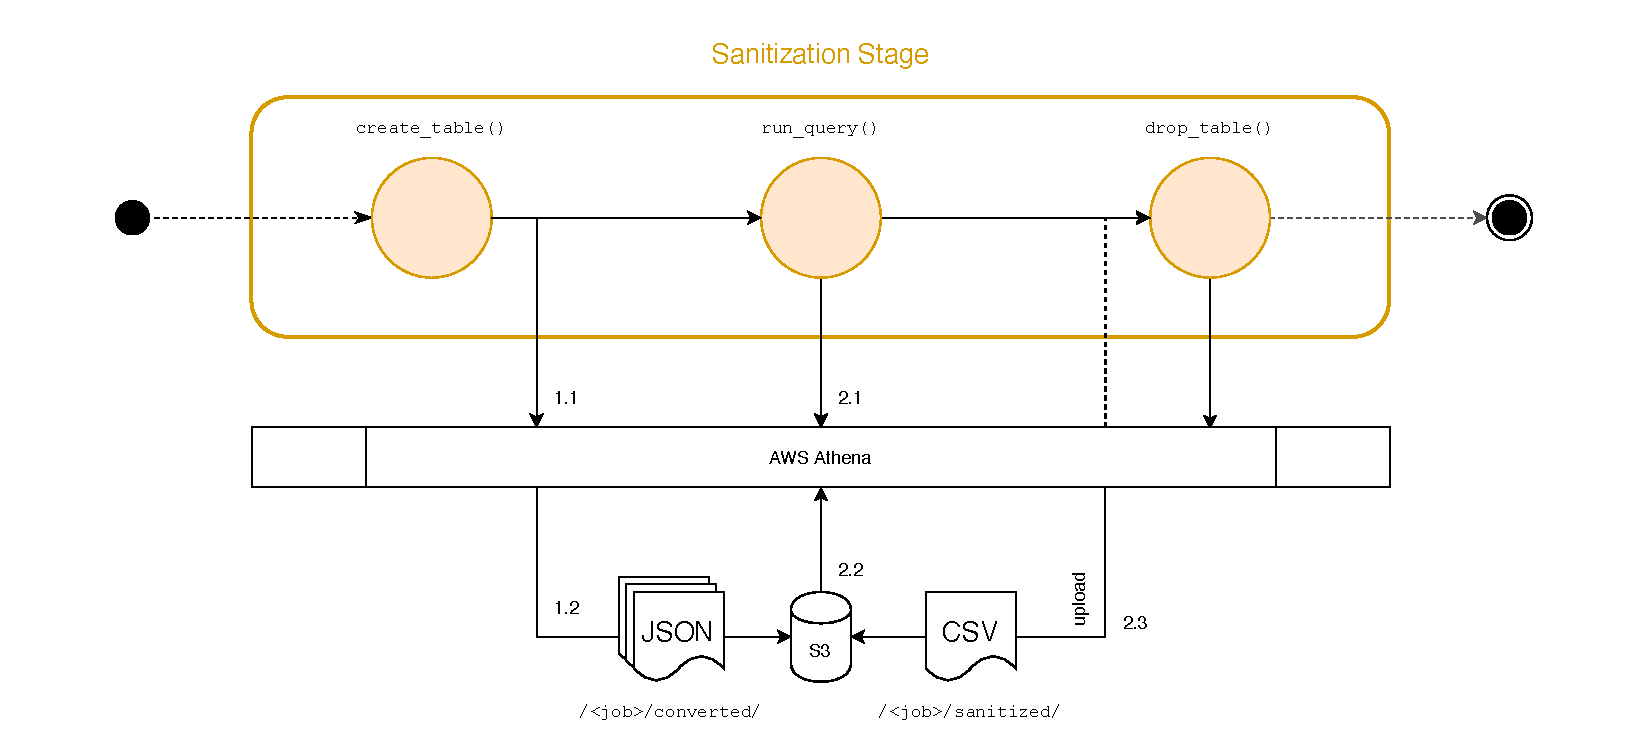
\includegraphics[width=\linewidth]{main-matter/img/3-3-3-sanitize}
	\caption{Sanitization Stage of the Data Pipeline}
	\label{fig:3-sanitize}	
\end{figure}

The currently provided \ac{json} files contain a significant amount of information which is not required for \ac{mba}. The data needs to be sanitized to only the required attributes for \ac{mba} and exported in \ac{csv} format.

Since each individual \ac{mba} has its own designated space in the data lake, the relational database table for each MBA needs to be created with its appropriate \ac{json} file location. Thus, Athena \ac{ddl} is used to create the table and insert each \ac{json} file as a row into the table.

After the table is populated, the Athena \ac{sql} query for \texttt{InvoiceNo}, \texttt{Description}, \texttt{ItemType}, and \texttt{Quantity} (cf. Source Code Excerpt \ref{src:3-athena-query}) results in the representation that is needed by the \ac{mba} engine. This query result is exported to the prepared-file directory of the job-specific data lake space. For the sake of a clean environment, the previously created table is dropped. The generated \ac{csv} file can now be used for \ac{mba}.

\subsection{\acs{mba} Stage}
Figure \ref{fig:3-mba} visualizes the \ac{mba} Stage.

\begin{figure}[h!]
	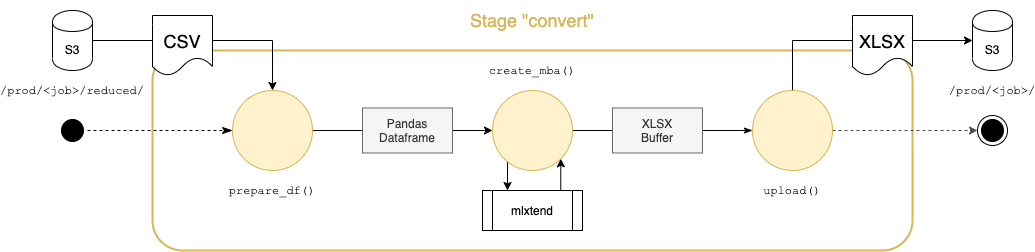
\includegraphics[width=\linewidth]{main-matter/img/3-3-4-mba}
	\caption{\acs{mba} Stage of the Data Pipeline}
	\label{fig:3-mba}	
\end{figure}

As mentioned in its own section, the \ac{csv} file is provided to the \ac{mba} engine. In case the data is not in correct order (horizontal or vertical, respectively), it is reordered in the process of creating the \texttt{pandas} data frame. \texttt{apriori} is applied on the data frame, which is then used to determine \texttt{association\_rules}. The \texttt{Quantity} attribute of the CSV file provides information on which items (i.e., \texttt{Description}s) where purchased in a transaction (identified by \texttt{InvoiceNo}), separated by \texttt{ItemType} \texttt{F} (i.e., food) and \texttt{N} (i.e., non-food). Both the food and non-food data frames and association rules need to be exported to a single Excel spreadsheet file. This functionality is also covered by \texttt{pandas} \cite{pandas}. This file is finally uploaded to the root directory of the current analysis job data lake space. At this point, one \ac{mba} data pipeline process is finished. 


\section{Comparison to Target Requirements}
From an infrastructure point of view, the preliminary solution meets the requirement of being implemented by means of \ac{aws} cloud services. On the contrary, the current architecture design is not server-less. More specifically, all analytics steps are performed on the same Airflow instance, resulting in bad scalability and a \ac{spof} dependency (cf. Figure \ref{fig:3-data-pipeline}). Additionally, since some steps inside the pipeline might have different performance requirements, the server-driven architecture could lead to bottlenecks for some stages and to overhead for others.

From a DataOps perspective, the solution at hand lacks fundamental implementation of state-of-the-art methodologies, e.g. \ac{vcs} support, \ac{cicd} automation, etc. These aspects need to be covered, taking the use case circumstances into consideration. Developing the solution needs to be done in individual, isolated environments in order not to contaminate the production-grade environment as well as other developers' environments within the project. This can be achieved by \ac{vcs} enablement. Additionally, since each pipeline stage is expected to be developed and maintained by different developers, the individual stages could have different requirements for their \ac{cicd} automation. Therefore, four individual DataOps \ac{cicd} pipelines need to be implemented by applying the different needs for every stage.

Finally, the current solution is entirely untested. This includes the absence of validating software tests as well as data quality checks within the solution. A use-case-specific testing framework based on the use case data definition and governance is required. This framework needs to be designed before it can be embedded inside the future DataOps processes of the solution.